\documentclass{article}
\usepackage{graphicx}
\usepackage{amsmath}
\usepackage{amssymb}
\usepackage[italicdiff]{physics}
\usepackage{enumerate}
\usepackage{microtype}
\DisableLigatures{encoding= *, family=*}
\usepackage{titlesec}
\usepackage{xfrac}
\setcounter{secnumdepth}{4}
\usepackage{xcolor}
\usepackage[bookmarks=false]{hyperref}
\usepackage{mathtools}
\usepackage{bigints}
\hypersetup{
    colorlinks=true,
    linkcolor=[RGB]{59 108 209},
    urlcolor=[RGB]{59 108 209}
}
\urlstyle{same}

\titleformat{\paragraph}
{\normalfont\normalsize\bfseries}{\theparagraph}{1em}{}
\titlespacing*{\paragraph}
{0pt}{3.25ex plus 1ex minus .2ex}{1.5ex plus .2ex}

\title{Wurtz Reaction}
\author{}
\date{}

\begin{document}
\maketitle
\section{Reaction and Mechanism}
\begin{center}

    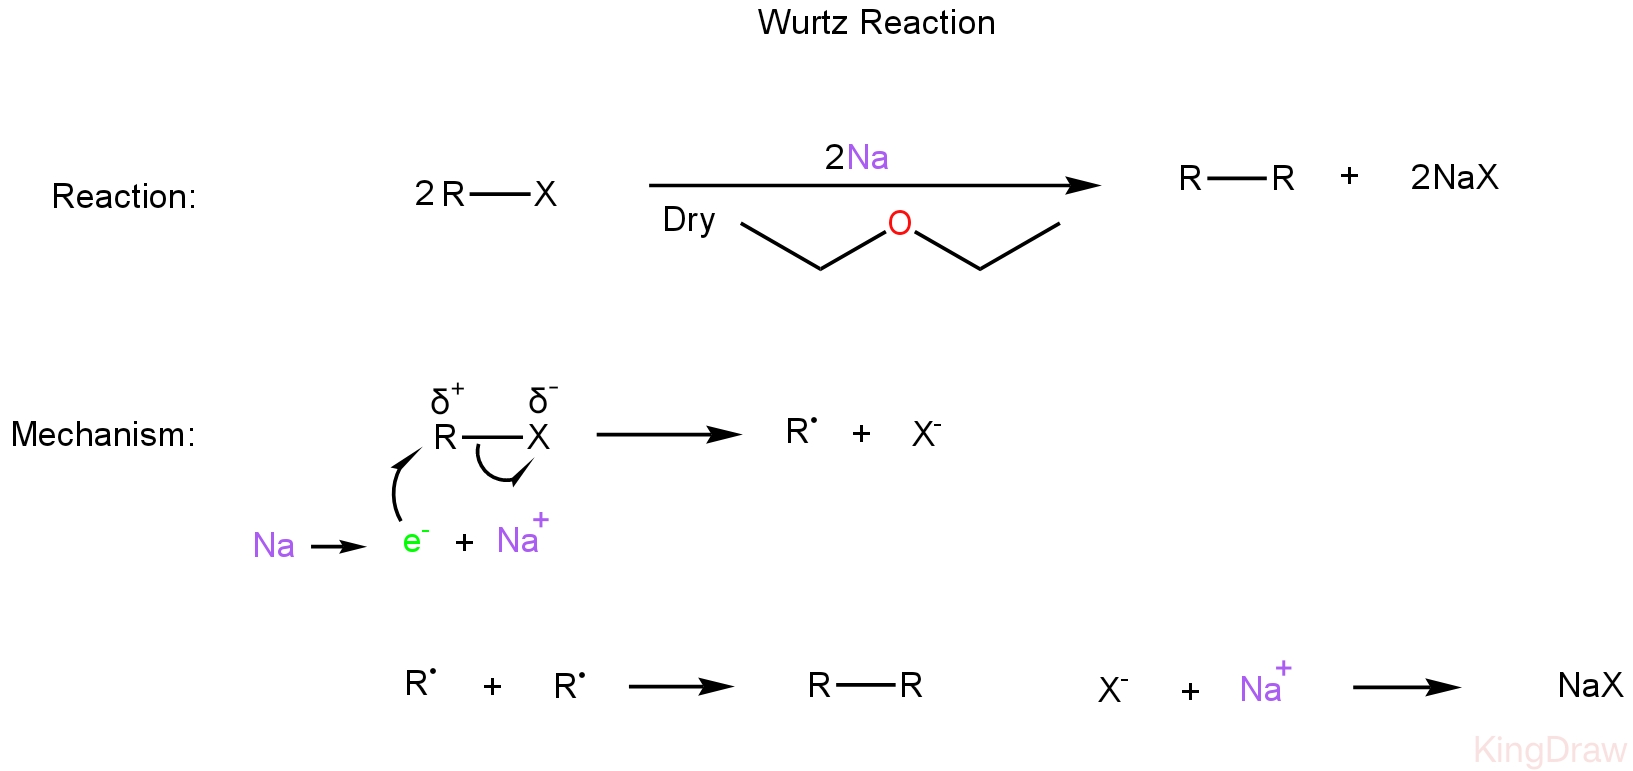
\includegraphics[scale=0.25]{WurtzReaction(1)_1722164749564.JPEG}
\end{center}

\section{Why dry $Et_{2}O$ is used instead of moisture?}
Water and Sodium metal react vigorously to form Sodium Hydroxide and evolve hydrogen gas, to avoid this reaction taking place dry environment is preferred.
\section{Why $Et_{2}O$ is used?}
$Et_{2}O$ is a PAS, hence it solvates only the cationic part (+).

\section{Reaction Observations}
\begin{enumerate}[i.]
    \item Free radical or $C^-$ obtained as intermediate.
    \item Breaking of $RX$ bond is RDS.
    \item $ROR$ for $RX$, $RI > RBr> RCl$
    \item $\textit{Stability of } R^\cdot \propto ROR $
    \item $RF$ doesn't react.
    \item $CH_{4}$ can never be obtained.
    \item Only symmetrical even number of $\prescript{12}{6}{C}$ obtained in very good yield.
    \item Unsymmetrical compound obtained in very poor yield.
\end{enumerate}

\end{document}